%performance evaluation
\section{Performance evaluation}
\justify
In this section we are going to evaluate our parallel approach, generate and comment some graphs and also implement a cut-off mechanism.
\justify
The execution time of the last version is 1.065s. If we compare it to the execution time of the serial version, 0.942s, we can see that the performance got a 13\% worse. This is caused by the serious overheads of task creation and synchronization plus the memory copy of each thread. In the following figure you can see the time diagram from paraver with a size of 4 and 8 threads.

\justify
In order to get a better performance and as we seen on previous laboratories, we are going to implement a cut-off mechanism.
\justify
We only have on pragma creating tasks, so the cut-off will be fairly easy to implement. To control how deep we are in the recursion tree we don't need to add an extra variable, since the \textit{j} parameter already gives us that information. We used this value to implement a final clause in our task creation pragma, so once it reaches a certain level it stops creating more tasks.   
\begin{lstlisting}
#pragma omp task final(j >= cutoff) mergeable
\end{lstlisting}
\justify
In order to obtain the optimal number for the cut-off value, we created a script that tried different values for a given number of threads.
\begin{lstlisting}[escapechar=@]
setenv OMP_NUM_THREADS 8
setenv OMP_WAIT_POLICY "passive"
setenv size 12
set depth_list = @"0 1 2 3 4 5 6 7 8 10 15 20 32 64 128 1023"@
set out = out.txt
rm -rf $out
rm -rf o
rm -rf ./elapsed.txt
foreach depth ( $depth_list )
    echo $depth >> $out
    ./nqueens-omp -n$size -c$depth >> o
    set result = `cat o | tail -n 4  | grep "Solution Count Time"
                  | cut -d' ' -f 5`
    echo $result >> $out
end
\end{lstlisting}

\clearpage
\justify
We ran this script changing the number of threads to obtain the following table:
\begin{table}[!h]
\begin{tabular}{|l|l|l|l|l|l|l|l|l|l|}
\hline
 & \multicolumn{9}{c|}{Cut-off value} \\ \cline{2-10} 
\multirow{\#Threads} & 1 & 2 & 4 & 6 & 8 & 16 & 32 & 64 & 512 \\ \hline
4 & 0.73 & 0.72 & \cellcolor[HTML]{C0C0C0}{\color[HTML]{333333} 0.71} & 0.81 & 1.33 & 2.03 & 2.03 & 2.04 & 2.0 \\ \hline
8 & 0.45 & 0.44 & \cellcolor[HTML]{C0C0C0}0.42 & 0.49 & 0.71 & 1.12 & 1.08 & 1.11 & 1.09 \\ \hline
12 & 0.38 & \cellcolor[HTML]{C0C0C0}0.34 & 0.36 & 0.41 & 0.51 & 0.83 & 0.81 & 0.85 & 0.86 \\ \hline
16 & 0.36 & 0.29 & \cellcolor[HTML]{C0C0C0}0.25 & 0.29 & 0.44 & 0.68 & 0.68 & 0.68 & 0.67 \\ \hline
\end{tabular}
\end{table}

\justify
We can observe that the optimum value of the cut-off variable is 4 in most cases. With this value and the same number of threads(8) than when we evaluated the omp version without cut-off, we obtain an execution time of 0.42s. This marks a speed up of 2.53 to the first parallel version and 2.24 to the serial version.
\justify
To finish evaluating the parallelization of the code, we are going to obtain the strong scallability plot from the last version; using a size of 13, 8 threads and a cut-off value 4.

\begin{figure}[!h]
    \centering
    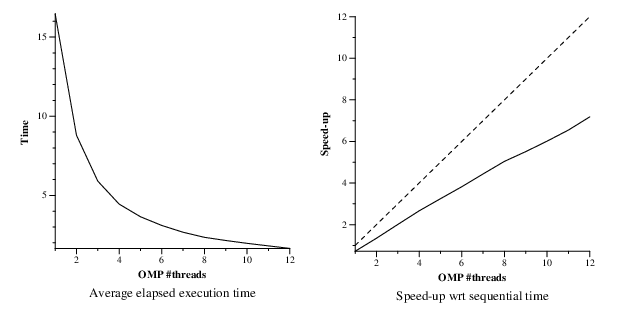
\includegraphics[width=0.78\textwidth]{strong.png}
    \caption{Strong speed-up plots}
    \label{fig:strong}
\end{figure}


\justify 
As it can be seen, the strong scallability is not as close to the ideal case as we are used to. This is caused by the overhead of the memory copying, the critical/atomic zones and the cut-off mechanism.

%FALTA : MIRAR QUANT CUTOFF VAM FER SERVIR PEL TEMPS 0.749 I MIRAR COM FER LO DEL OPTIMAL..CREC QUE TENIEM LSCRIPT FET JA